\section{Passive exterior reception and exact identifiability}\label{sec:exterior}
The C6 rule is a separate adoption from SRG-06.~\cite{SRG06} At a fixed off-circle centre $X$ with known orthonormal frame $B$, let $d_X(s)=\norm{X-\Gamma(s)}$. For an independent speed $c_e>0$ and common dimensionless gain $g_o>0$, define
\begin{equation}\label{eq:C6}
 \begin{aligned}
 U(X,t)&=\frac{g_o}{4\pi}\int_0^L\frac{p(s,t-d_X(s)/c_e)}{d_X(s)}\dd s,\\
 V(X,t)&=\frac{g_o}{4\pi}\int_0^L\frac{r(s,t-d_X(s)/c_e)\hat t(s)}{d_X(s)}\dd s,\qquad
 Y_X=(U,B\tr V).
 \end{aligned}
\end{equation}
The straight-line delay, $1/d$ weight, tangent encoding and absence of screening or loading are assumptions. No nearest-point projection, spoke or equality of outer and local azimuths is used. The vector $r\hat t$ is not carrier flux $j$, native $C$, or an assigned material current. The full miniature remains geometrically present, while the sensor is idealized as centre-sampled.

\subsection{Distance, history domain and covariance}
Write $X-B_0=\xi u+\zeta\ez+\upsilon v$, $q=(\xi^2+\zeta^2)^{1/2}$ and, for $q>0$, $\phi=\operatorname{atan2}(\zeta,\xi)$. Then
\begin{equation}\label{eq:distance}
 d_X^2(\chi)=q^2+\upsilon^2+R^2-2Rq\cos(\chi-\phi),\qquad
 d_{\min,\max}=\sqrt{(q\mp R)^2+\upsilon^2}.
\end{equation}
This follows by expanding the squared norm; cosine ranges between $-1$ and $1$. For $q=0$ the distance is constant. Every admitted site has $q>0$, and the array minimum is $2-K-R=0.7068378998\ldots>0$, attained at R1:00. Thus the coarse triangle-inequality clearance is attained, not strictly improved. The distance spread is at most the circle diameter $2R$.

\begin{theorem}[Bounded causal history map]\label{thm:history}
Let $X\notin\Gamma$ and $I_*=[t_0,t_1]$. With
$J_*=[t_0-d_{\max}/c_e,t_1-d_{\min}/c_e]$, C6 defines a bounded linear map from $L^2(J_*\times\Gamma;\R^2)$ to $L^2(I_*;\R^4)$, satisfying
\begin{equation}\label{eq:historybound}
 \norm{Y_X}_{L^2(I_*)}
 \le\frac{g_o}{4\pi}\left(\int_0^L d_X^{-2}\dd s\right)^{1/2}
 \norm{(p,r)}_{L^2(J_*\times\Gamma)}
 \le\frac{g_o\sqrt L}{4\pi d_{\min}}\norm{(p,r)}_{L^2(J_*\times\Gamma)}.
\end{equation}
Continuous time into $H^1_{\rm per}$ supplies pointwise records. The map is causal and leaves C1 and its storage account unchanged.
\end{theorem}
\begin{proof}
For each fixed $s$, translate the time variable by $d_X(s)/c_e$. Its Jacobian is one, and the shifted output interval lies in $J_*$. The norm of the vector integrand $(p,B\tr(r\hat t))$ is $\sqrt{p^2+r^2}$, because $B$ is orthogonal and $\norm{\hat t}=1$. Minkowski's integral inequality followed by Cauchy--Schwarz in $s$ therefore gives the first bound; replacing $d_X^{-1}$ by $d_{\min}^{-1}$ gives the second. This argument also shows that almost-everywhere equivalent histories give the same almost-everywhere output: apply the time change at almost every $s$ and Fubini. For the pointwise assertion, the embedding of periodic one-dimensional $H^1$ into continuous functions and continuous time dependence provide a jointly continuous representative on compact intervals. The delay is positive, so only earlier inputs enter. Linearity is immediate, and no field or work equation contains $Y_X$.
\end{proof}

The history norm in \eqref{eq:historybound} cannot generally be replaced by $E(t)$ at one instant: different arclengths are sampled at different times. An eternally harmonic free preparation has no first arrival; multiplying it by a step does not preserve the unforced PDE. Source-driven histories instead use the causal solution below.

For a common orthogonal transformation $T_o$ and translation $b_o$, transform $(\Gamma,X,\hat t,B)$ to $(T_o\Gamma+b_o,T_oX+b_o,T_o\hat t,T_oB)$. Distance is unchanged, $U'=U$ and $V'=T_oV$, so the local components agree, including under improper transformations. For arclength reversal set $p'(s,t)=p(L-s,t)$, $r'(s,t)=-r(L-s,t)$ and $\hat t'(s)=-\hat t(L-s)$. The product $r'\hat t'$ is geometrically unchanged. Relabelling the coordinate does not physically exchange the drives.

The vector always lies in $\operatorname{span}(u,\ez)$, so $(B\tr v)\tr(B\tr V)=0$. Four reported entries provide one scalar and at most two vector directions. Duplicated sites add repeated rows, not states. The formal $g_o=0$ limit deletes records without changing the field. The $c_e\to\infty$ limit is simultaneous weighted integration, distinct from the uniform map of Paper I. A common extra delay multiplies a phasor by a unit complex factor and preserves its singular values; it does not remove differential delay.

\subsection{Circular reduction and a finite-delay rank proof}
Use the free family \eqref{eq:freefamily} with $\omega=c/R$. Define $\beta=\omega/c_e$ and $\nu=\beta R=c/c_e$. For unit exterior gain set
\begin{equation}\label{eq:Q}
 h_\pm=\frac1{4\pi}\int\frac{e^{\mp\ii\chi-\ii\beta d}}d\dd s,\quad
 v_\pm=\frac1{4\pi}\int\frac{e^{\mp\ii\chi-\ii\beta d}\hat t}d\dd s,
 \quad Q_X=\begin{pmatrix}h_+&h_-\\B\tr v_+&-B\tr v_-\end{pmatrix}.
\end{equation}
Then $\widehat Y_X=g_oQ_X(a_+,a_-)\tr$. The negative temporal delay phase and the minus in the second directional column have different origins; both are essential.

\begin{theorem}[Moment reduction and singular values]\label{thm:reduction}
For $q>0$, put $\alpha=\chi-\phi$, $e_q=\cos\phi\,u+\sin\phi\,\ez$, $e_\perp=-\sin\phi\,u+\cos\phi\,\ez$, and
\begin{equation}\label{eq:moments}
 (H,S_m,C_m)=\frac R{4\pi}\int_0^{2\pi}\frac{e^{-\ii\beta d(\alpha)}}{d(\alpha)}
 (\cos\alpha,\sin^2\alpha,\cos^2\alpha)\dd\alpha.
\end{equation}
For $z_\pm=e^{-\ii\phi}a_+\pm e^{\ii\phi}a_-$,
\begin{equation}\label{eq:reduction}
 \widehat U=g_oHz_+,\qquad
 \widehat V=g_o(\ii S_me_qz_++C_me_\perp z_-).
\end{equation}
The full map has singular values, in either order,
\begin{equation}\label{eq:singularvalues}
 \sqrt2g_o\sqrt{|H|^2+|S_m|^2},\qquad \sqrt2g_o|C_m|.
\end{equation}
For the vector map alone they are $\sqrt2g_o|S_m|,\sqrt2g_o|C_m|$.
\end{theorem}
\begin{proof}
The distance is even in $\alpha$, and $\hat t=-\sin\alpha\,e_q+\cos\alpha\,e_\perp$. Expanding $e^{\mp\ii\chi}=e^{\mp\ii\phi}(\cos\alpha\mp\ii\sin\alpha)$ eliminates odd integrands. Consequently $h_\pm=e^{\mp\ii\phi}H$ and $v_\pm=e^{\mp\ii\phi}(\pm\ii S_me_q+C_me_\perp)$. Substituting the minus of the second vector column proves \eqref{eq:reduction}. The two output vectors multiplying $z_+$ and $z_-$ are Hermitian-orthogonal. The sum/difference input matrix has Gram $2I_2$. Multiplying by the isometric local frame leaves norms unchanged, yielding \eqref{eq:singularvalues} and the vector-only result. At $q=0$, choose any $\phi$; the constant kernel gives $H=0$ and the same singular-value formula.
\end{proof}

\begin{theorem}[Nonvanishing in a sufficient delay range]\label{thm:sector}
For any off-circle $X$ and $0\le\nu<\pi/2$, the full and vector maps have complex rank two. For $q>0$, also $H\ne0$. In particular,
\begin{equation}\label{eq:sectorbound}
 |S_m|,|C_m|\ge\frac{R\cos\nu}{4d_{\max}},\qquad
 |H|\ge\frac{R^2q\cos\nu}{4d_{\max}^3},\qquad
 \sigma_{\min}(g_oQ_X)\ge\frac{\sqrt2g_oR\cos\nu}{4d_{\max}}>0.
\end{equation}
The two admitted comparison settings $\nu=0,1$ satisfy this range. No all-frequency assertion is made.
\end{theorem}
\begin{proof}
At $\beta=0$, the weights $1/d$ are positive and the nonnegative functions $\sin^2\alpha,\cos^2\alpha$ each have positive integral, so both moments are positive. At finite delay a different argument is necessary. Let $d_*=(d_{\min}+d_{\max})/2$ and $\delta=\beta(d_{\max}-d_{\min})/2\le\nu$. Rotate each moment by $e^{\ii\beta d_*}$. The real part of its integrand is at least $\cos\delta$ times its nonnegative undelayed weight. Since $\int_0^{2\pi}\sin^2\alpha\dd\alpha=\int_0^{2\pi}\cos^2\alpha\dd\alpha=\pi$, this gives the first two nonzero-moment bounds.

To treat $H$, integrate the derivative of $\sin\alpha\,e^{-\ii\beta d}/d$ over one period. From $d'=Rq\sin\alpha/d$ one obtains
\begin{equation}\label{eq:Hparts}
 H=\frac{R^2q}{4\pi}\int_0^{2\pi}
 \frac{\sin^2\alpha\,e^{-\ii\beta d}(1+\ii\beta d)}{d^3}\dd\alpha.
\end{equation}
The continuous phase $\psi(d)=-\beta d+\arctan(\beta d)$ has derivative
$-\beta^3d^2/(1+\beta^2d^2)$ of magnitude at most $\beta$. Its phase spread is at most $2\nu$. Rotation by the midpoint of that phase interval therefore makes the real part at least $\cos\nu$ times the modulus. Using $|1+\ii\beta d|\ge1$ and $d\le d_{\max}$ proves the $H$ bound. The singular-value bound now follows from Theorem~\ref{thm:reduction}. This argument uses a complex sector, not a false positivity claim for delayed weights.
\end{proof}

A separate perturbation estimate, useful when the sector condition is not the chosen test, is
\begin{equation}\label{eq:perturb}
 \norm{g_oQ_\beta-e^{-\ii\beta d_*}g_oQ_0}_2
 \le\frac{g_o\delta}{2\pi}\int_\Gamma d^{-1}\dd s
 \le\frac{g_o\delta L}{2\pi d_{\min}}.
\end{equation}
To prove it, subtract the two integrands in \eqref{eq:Q}, use $|e^{-\ii x}-1|\le|x|$ and note that the two-column scalar-plus-vector integrand has Frobenius norm $2$. Integrating bounds the operator norm. If the bound is below $\sigma_{\min}(g_oQ_0)$, the inequality $\norm{(Q_0+E)x}\ge\norm{Q_0x}-\norm E\norm x$ proves rank preservation. The condition can be conservative; Theorem~\ref{thm:sector} settles $\nu=1$ directly.

\subsection{What height changes, and radius cannot change}
\begin{theorem}[Scalar obstruction and height discrimination]\label{thm:height}
At every off-circle equatorial site, for every exterior delay, $h_+=h_-$. Thus any coplanar scalar array conflates T+, T- and S45 of Table~\ref{tab:free}, with their equal storage and common calibration. No increase in coplanar radius removes this null. At $\nu=0,1$, the fixed mirror pair H+1:00/H-1:00 and each off-height H ring have scalar complex rank two on the two-amplitude family. At every individual retained site the vector/full map has rank two.
\end{theorem}
\begin{proof}
At height zero the distance is even in $\chi$; the sine part of the scalar integral vanishes, giving $h_+=h_-$. Equivalently $\phi=0$ or $\pi$ at fixed sites. The source sums $a_++a_-$ for T+, T- and S45 all equal $A_0/\sqrt2$, so their entire scalar histories coincide. S0 has sum $A_0$ and differs only by the known factor $\sqrt2$.

At nonzero height one scalar row is $H(e^{-\ii\phi},e^{\ii\phi})$. Two such rows are independent when $H_1H_2\sin(\phi_2-\phi_1)\ne0$. For the stated mirror pair their determinant is $-2\ii g_o^2H^2\sin(2\phi)$, with
\begin{equation}\label{eq:mirrorminor}
 \sin(2\phi)=\frac{2(3-K)a}{(3-K)^2+a^2}\ne0.
\end{equation}
The moments are nonzero by Theorem~\ref{thm:sector}. On any fixed off-height ring, sites 00 and 03 have respectively $\xi=3-K$ and $\xi=-K$, with the same nonzero height. Their $(\xi,h)$ vectors are not parallel, since their determinant is $3h\ne0$; their two scalar phases therefore give an independent pair. The within-site vector/full assertion is already proved by the sector theorem.
\end{proof}

For height reflection $F=\diag(1,1,-1)$ in world coordinates, substitution $\chi\mapsto-\chi$ gives $h_\pm(FX)=h_\mp(X)$ and $v_\pm(FX)=-Fv_\mp(X)$. The frames are unchanged above and below, hence
\begin{equation}\label{eq:mirrorQ}
 Q_{-h}=\diag(1,1,-1,1)\,Q_h
 \begin{pmatrix}0&1\\1&0\end{pmatrix}.
\end{equation}
This is symmetry of reception at matched centres, not a claim that all folded miniature surfaces are literal mirror copies. A fixed selected circle also breaks central $C_3$ invariance unless the source pair and circle are rotated together. Distance and phase depend nonlinearly on site angle; two source amplitudes do not imply only two site Fourier indices.

\subsection{Retained numerical matrices and their qualification}\label{sec:numerics}
Table~\ref{tab:Qdata} transcribes the accepted SRG-06 matrices; $g_o=1$ is common to all rows. No spatial quadrature is repeated here. Exact zeros follow from symmetry, not a floating threshold. The uniform analytic singular-value lower bound across these sites/settings is $0.0193600993g_o$; the retained computed minimum is $0.0262859195g_o$.
\begin{table}[htbp]\centering\small
\begin{tabular}{lccrr}\toprule
Stack & Scalar rank & Full rank & Scalar $\sigma_{\min}$, $0/1$ & Full $\sigma_{\min}$, $0/1$\\\midrule
H$\pm2$, each &2&2& .00946563 / .05460398&.21704541 / .19008006\\
H$\pm1$, each &2&2& .00521440 / .02915133&.22368205 / .18961117\\
H0=R2 &1&2&0 / 0&.22604866 / .18924224\\
R1 &1&2&0 / 0&.35548794 / .30194822\\
R3 &1&2&0 / 0&.16712416 / .13941997\\
H (60 sites)&2&2&.01927634 / .09275635&.49542995 / .42564193\\
R (36 sites)&1&2&0 / 0&.45321095 / .38265295\\
Union (84 sites)&2&2&.01927634 / .09275635&.63226023 / .54016822\\\bottomrule
\end{tabular}
\caption{Inherited complex-phasor sensitivities at $\nu=0$ and $1$, in that order. The union deduplicates H0/R2. Numerical summaries carry a $10^{-11}$ allowance; these are not directed-rounded enclosures.}\label{tab:Qdata}
\end{table}

The retained integrals used periodic trapezoids with $N=128,256,512$ at 60 decimal digits, with independent 80-digit original-angle checks at four predeclared sites. For a strip half-width $\sigma=1/4$, put $A_d=q^2+\upsilon^2+R^2$ and $m=A_d-2Rq\cosh\sigma>0$. The principal distance square root is analytic in this strip, since its squared real part is positive there. Each direct scalar/world-plane integrand is bounded by
\begin{equation}\label{eq:quadbound}
 M_*=\frac{Re^\sigma\cosh\sigma}{4\pi\sqrt m}
 \exp\!\left(\frac{\nu\sqrt{A_d+2Rq\cosh\sigma}}R\right),
 \qquad e_{\rm entry}\le\frac{4\pi M_*}{e^{N\sigma}-1}.
\end{equation}
For completeness, shifting the Fourier coefficient contour to the two strip boundaries gives coefficient modulus at most $M_*e^{-|n|\sigma}$. The periodic trapezoid retains precisely the coefficients at multiples of $N$; summing the two geometric alias tails and multiplying by $2\pi$ gives \eqref{eq:quadbound}. Six independent scalar/world-plane entries yield a Frobenius error at most $\sqrt6e_{\rm entry}$, preserved under the frame isometry.

The maximum retained $N=512$ truncation bound is $2.114\times10^{-52}$, and the largest 256-to-512 difference is $1.125\times10^{-62}$. These numbers do not certify floating arithmetic. The original mpmath calculation was not interval arithmetic; its disclosed arithmetic allowance is $10^{-45}$, serialized matrix-entry allowance $10^{-14}$ and matrix-summary allowance $10^{-11}$. The exact rank results rest on the written proofs, independently of these numerical allowances.

\begin{figure}[htbp]\centering
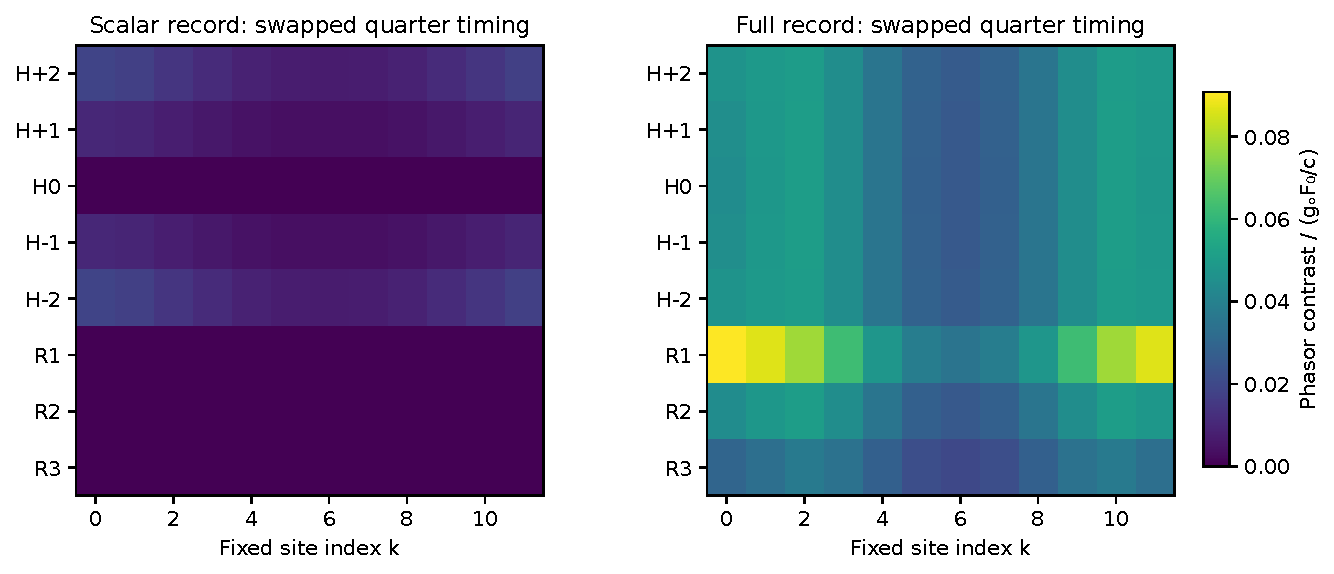
\includegraphics[width=\textwidth]{figures/exterior.pdf}
\caption{Scalar versus full exterior contrast, redrawn from retained SRG-06--08 data. Equatorial scalar rows have exact zero contrast for exchanged direction/timing; directional records remain distinct. Horizontal indices are fixed sites, not time. Common calibration is retained, and no entry is normalized separately.}\label{fig:exterior}
\end{figure}

\subsection{Phasors, snapshots, calibration and squared records}\label{sec:information}
Complex rank two identifies two complex amplitudes with a known clock and gain, equivalently their full-period records at known nonzero frequency. An unknown common nonzero complex factor leaves the ratio $a_-/a_+$ identifiable after a rank-two inverse, but removes absolute scale and common phase. Its modulus gives $\Jflux/(cE)$ for the mean-free family. If separate unknown factors multiply each scalar site, they can absorb the height phase contrast site by site. A full single site still has a projective inverse when one factor is common to all its channels; independent channel factors or an unknown frame remove that guarantee.

One real snapshot instead maps four real amplitude coordinates through $[\Re Q,-\Im Q]$, up to a common time phase. One site has at most three real channels and cannot invert four real unknowns. The retained finite stack results are:
\begin{table}[htbp]\centering
\begin{tabular}{lcc}\toprule
Stack & Scalar real rank, $\nu=0/1$ & Full real rank, $\nu=0/1$\\\midrule
Each off-height H ring &2 / 4&4 / 4\\
Each equatorial ring &1 / 2&3 / 4\\
H or unique union &2 / 4&4 / 4\\
R &1 / 2&3 / 4\\\bottomrule
\end{tabular}
\caption{Inherited snapshot classifications for the all-time first-harmonic family. Finite-delay full-rank statements here are finite numerical findings; the smallest reported nonzero singular value exceeds .005.}\label{tab:snapshots}
\end{table}
At zero delay, the scalar snapshot contains only the two real spatial coefficients of $p$, and an equatorial vector record misses one real coefficient of $r$, explaining the exact upper bounds. Retarded samples can contain additional quadratures in this assumed family. This is not instantaneous reconstruction of arbitrary histories.

\begin{proposition}[Squared-record blindness]\label{prop:power}
For T+ and T-, scalar phasor magnitudes and full phasor squared norms agree at every off-circle site and every delay. For the standing controls,
\begin{equation}\label{eq:scalarpower}
 |\widehat U_{S0}|^2=g_o^2A_0^2|H|^2\cos^2\phi,\qquad
 |\widehat U_{S45}|^2=g_o^2A_0^2|H|^2\cos^2(\phi-\pi/4).
\end{equation}
Individual directional-component period mean squares can differ at finite delay.
\end{proposition}
\begin{proof}
For either traveller, $|z_+|=|z_-|=A_0/\sqrt2$. Orthogonality in \eqref{eq:reduction} makes scalar and total squared norms identical. Substituting the two standing amplitudes gives the cosine factors in \eqref{eq:scalarpower}. For a real local component, set $q_j=(B\tr e_q)_j$ and $t_j=(B\tr e_\perp)_j$. The two vector column entries differ by the sign of the $C_mt_j$ term. Expanding their squared moduli and multiplying by the traveller amplitude square and the period factor $1/2$ gives
\begin{equation}\label{eq:componentpower}
 \langle Y_{j,T+}^2\rangle-\langle Y_{j,T-}^2\rangle
 =g_o^2A_0^2\Re(\ii S_m\overline{C_m})q_jt_j.
\end{equation}
At zero delay the moments are real, so this vanishes. Summing components also gives zero because $e_q\cdot e_\perp=0$.
\end{proof}
At H+1:00 and $\nu=1$, the inherited component differences $(U,V_1,V_2,V_3)$ are $(0,-8.21792406\times10^{-5},+8.21792406\times10^{-5},0)$ for $g_o=A_0=1$. At equatorial sites the products $q_jt_j$ vanish in the retained frames. These are calibrated readout statistics, not emitted or absorbed power.

\subsection{Causal composition and possible arrival}\label{sec:causality}
From zero preparation at $t_0$, substitution of \eqref{eq:characteristics} into C6 gives
\begin{equation}\label{eq:composition}
 \begin{split}
 Y_X(t)=\frac{g_o}{8\pi}\sum_{j=\pm}\sum_{\sigma=\pm1}
 \int_\Gamma\frac{1}{d_X(s)}\binom{1}{\sigma B\tr\hat t(s)}\hspace{-1mm}
 \int_{t_0}^{t-d_X(s)/c_e}
 b_j\big(s-\sigma c[t-d_X(s)/c_e-u]\big)f_j(u)\dd u\dd s .
 \end{split}
\end{equation}
An inner integral with upper endpoint below $t_0$ is zero. Compact forcing can also truncate its upper endpoint at switch-off. The $1/2$ splitting follows from the two characteristic conversions and is not an adjustable gain.

\begin{proposition}[Support-arrival infimum]\label{prop:arrival}
For source support $S_j$ beginning at $t_0$, the first possible support arrival obeys
\begin{equation}\label{eq:arrival}
 t_0+\inf_{u\in S_j,\ s\in\Gamma,\ \sigma=\pm1}
 \left\{\frac{D_\sigma(u,s)}c+\frac{d_X(s)}{c_e}\right\}.
\end{equation}
If $c\le c_e$, this infimum equals $t_0+\inf_{u\in S_j}d_X(u)/c_e$.
\end{proposition}
\begin{proof}
The inner source integrand in \eqref{eq:composition} can contribute only after a characteristic has travelled from its support to $s$, followed by the exterior delay from $s$ to $X$. Taking the least directed arc and then the infimum gives \eqref{eq:arrival}; further windings add $L/c$. For $c\le c_e$, arc length exceeds chord length, so
\[
 \frac{D_\sigma(u,s)}c+\frac{d_X(s)}{c_e}
 \ge\frac{\norm{\Gamma(s)-\Gamma(u)}+d_X(s)}{c_e}
 \ge\frac{d_X(u)}{c_e}.
\]
Choosing $s=u$ gives equality of the infima. If $c>c_e$, the first inequality need not hold, and no such reduction is asserted.
\end{proof}
Tent edges, smooth source onset, zero integration length and scalar/vector cancellations can prevent nonzero measurement at the threshold. A parity-blind channel may remain zero forever. The calculation is about finite support, not a contact-centre shortcut. C6 changes no term in $\dot E$; neither a squared record nor its sum is a debit from the carrier.
